% !TeX spellcheck = de_DE
% !TeX encoding = UTF-8
% !TeX spellcheck = en_US
% !BIB TS-program = biber
% basic packages and document settings
\documentclass[a4paper,12pt]{article}
\usepackage[english]{babel}
\usepackage[utf8]{inputenc}
\usepackage[T1]{fontenc}
\usepackage[a4paper]{geometry}
\geometry{top = 30mm, bottom = 25mm, left = 25mm, right = 25mm}
\usepackage{setspace}
\onehalfspacing
\raggedbottom
\pdfcompresslevel9

% mathmode-related packages
\usepackage{mathtools}
\usepackage{physics}
\usepackage{amsmath}
\usepackage{amsthm}
\usepackage{amsbsy}
\usepackage{mathrsfs}
\usepackage{amssymb}
\usepackage{amstext}
\usepackage{amsfonts}
\usepackage{tikz}
\usepackage{siunitx}
%\usepackage{IEEEtrantools}

% misc
\usepackage{esdiff}
\usepackage{multirow}
\usepackage{blindtext}
\usepackage{todonotes}
\usepackage{abstract}
\usepackage{appendix}
\usepackage[bottom]{footmisc}
\usepackage{listings}
\usepackage{dashrule}

% graphics and floats
\usepackage{graphicx}
\graphicspath{{../Figures/}}
\usepackage{tikz}
\usepackage{float}
\usepackage{wrapfig}
%\usepackage{subfloat}
\usepackage{subcaption}
%\usepackage{caption}
\usepackage[rightcaption]{sidecap}
\usepackage{tabularx}
\usepackage{adjustbox}
%\usepackage{svg}
\usepackage{epstopdf}
\usepackage{grffile}	% handle file names with dots, spaces etc.
%\usepackage{flafter}
\usepackage{rotating}
%\usepackage{floatrow}
%\floatsetup[figure]{capposition=beside,capbesideposition={top,right}}

%\usepackage{epstopdf}
%\epstopdfDeclareGraphicsRule{.pdf}{png}{.png}{convert #1 \OutputFile}
%\AppendGraphicsExtensions{.pdf}

% packages requiring setup arguments

\usepackage{xcolor}
%\definecolor{rwth-dark}{HTML}{176daf}
\definecolor{rwth-dark}{RGB}{0,84,159}
%\definecolor{rwth-light}{HTML}{8abae3}
\definecolor{rwth-light}{RGB}{142,186,229}

%/**
%* Generated by Gpick 0.2.5
%* RWTH Dark: #176daf, rgb(23, 109, 175), hsl(32, 43%, 69%)
%* RWTH Light: #8abae3, rgb(138, 186, 227), hsl(195, 73%, 89%)
%*/

\usepackage{hyperref}
\hypersetup{hidelinks=true,colorlinks=true,allcolors=rwth-dark}
\usepackage[nameinlink,capitalise]{cleveref}
%\usepackage[hyphens]{url}
%\urlstyle{sf}
%\usepackage{breakurl}


% header & footer settings
\usepackage{fancyhdr}
\pagestyle{fancy}
%\renewcommand{\chaptermark}[1]{\markboth{#1}{}} % with this we ensure that the chapter and section headings are in lowercase.
\renewcommand{\sectionmark}[1]{\markright{\thesection\ #1}}
\fancyhf{} % delete current header and footer

%\fancyhead[LE,RO]{\large\thepage}
\fancyhead[L]{\large\rightmark}
\fancyhead[R]{\large\thepage}

\renewcommand{\headrulewidth}{0.3pt}
\renewcommand{\footrulewidth}{0pt}
%\addtolength{\headheight}{0.5pt} % space for the rule

\fancyfoot[C]{\thepage}

\fancypagestyle{plain}
{
	\fancyhead{} % get rid of headers on plain pages
	\renewcommand{\headrulewidth}{0pt} % and the line
}

% ========== command definitions =================================
\newcommand{\Thickline}{\rule{\linewidth}{0.4mm}}
\newcommand{\Thinline}{\rule{\linewidth}{0.1mm}}

\newcommand{\id}{\, \mathrm{d}}

\definecolor{codegray}{gray}{0.9}
\newcommand{\code}[1]{\colorbox{codegray}{\texttt{#1}}}

\newcommand{\skippage}{\clearpage{\thispagestyle{empty}\cleardoublepage}}

\def\@esphack{%
	\relax
	\ifhmode
	\spacefactor\@savsf
	\ifdim\@savsk>\z@
	\ignorespaces
	\fi
	\fi}

\title{\LARGE title}
\date{}


\begin{document}
	
\begin{titlepage}
	\thispagestyle{empty}
	\newgeometry{top=20mm, left=20mm, right=20mm, bottom=20mm}
	
%	\begin{minipage}{0.35\textwidth}
%		\begin{flushleft}
%
%
%		\end{flushleft}
%	\end{minipage}
%	\hfill
%	\begin{minipage}{0.65\textwidth}
%		\begin{flushright}
%
%		\end{flushright}
%	\end{minipage}
	
%	\vspace*{\fill}
	\hspace{0pt}
	\vspace{2cm}
	\begin{center}
%		\Thickline
%		\vskip -0.5cm
%		\Thinline
		\hdashrule{\linewidth}{1pt}{}
		\vskip -0.5cm
		\hdashrule{\linewidth}{0.5pt}{}
		
		\vspace{0.5cm}
		\Huge{ \textbf{ T7 \\}}
		\LARGE{ \textbf{Gaseous ionisation detectors and statistics} } 
		
		\hdashrule{\linewidth}{0.5pt}{}
		\vskip -0.95cm
		\hdashrule{\linewidth}{1pt}{}
%		\Thinline
%		\vskip -0.9cm
%		\Thickline 
		
		\vspace{3cm}
		\Large{\textbf{ Group 14 \\}}
		\Large{Heithem Assili, 368441 \\ Alexandre Drouet, 355095 \\ Olexiy Fedorets, 356615 \\}
		\vspace{1cm}
		\Large{\textsl{ Date of experiment: 14.03.2019 \\ Submission date: 28.03.2019}}
		
	\end{center}
	\vfill
%	\vspace*{\fill}
	
\end{titlepage}
	
	
	
%\skippage
\pagenumbering{roman}
\thispagestyle{plain}

\tableofcontents
%	\newpage
\newpage
\listoffigures

%\begingroup
%\let\cleardoublepage\relax
%\let\clearpage\relax
\listoftables
%\endgroup
%\listoftables

\skippage

\pagenumbering{arabic}
\setcounter{page}{1}
\restoregeometry
\thispagestyle{fancy}


\section{Introduction}

The goal of this experiment is to get aquainted with gas detectors and to learn how to operate them. Furthermore we want to measure statistical distributions related to decay processes.

\subsection{Gas detectors}

\subsection{Statistics}

\section{Measurments with the Geiger counter}

\subsection{Procedure}

First we placed a Sr90-Probe in a lead chamber and measured the count rate's dependence on the voltage.

Next we checked the intensity of the background, by measuring the pulse rate without a probe in the chamber and found it to be \SI{4}{s^-1}

\subsection{Analysis}

\subsubsection{Characterization of dead time}

First of all we generated a puls of $1\,MHz$ with the generator
that is linked to the variable dead time stage($2\,ms$,$1\mu\,s$) and wrote down the count (counts over $2\,s$ measured $3$ times).
With
\begin{equation}
N =\frac{n_1}{1-n_1\cdot\tau_1}=\frac{n_2}{1-n_2\cdot\tau}
\end{equation}
we can correct the stage if we consider that the smaller stage is correct 
with a measured count rate of $10^6$ for $1\mu\,s$ and 
$519.67\pm0.07$ for $2\,ms$ we get a corrected stage of $1.92\,ms$.

Now we can calculate with the same method the resolution time of the GM-counter.
We consider that the real stage is between $\SI{1}{\micro s}$ and $\SI{2}{ms}$ with
\begin{equation}
\tau =\frac{1}{n_2}-\frac{1}{n_1}+\tau_1
\end{equation}
and $n_2=\SI{179.6\pm0.6}{s^{-1}}$ and $n_1=\SI{246.0\pm1.8}{s^{-1}}$ we got a resolution time of $\tau=\SI{422\pm35}{ms}$.

\subsubsection{Stever diagram}

%\begin{figure}[H]
%\centering
%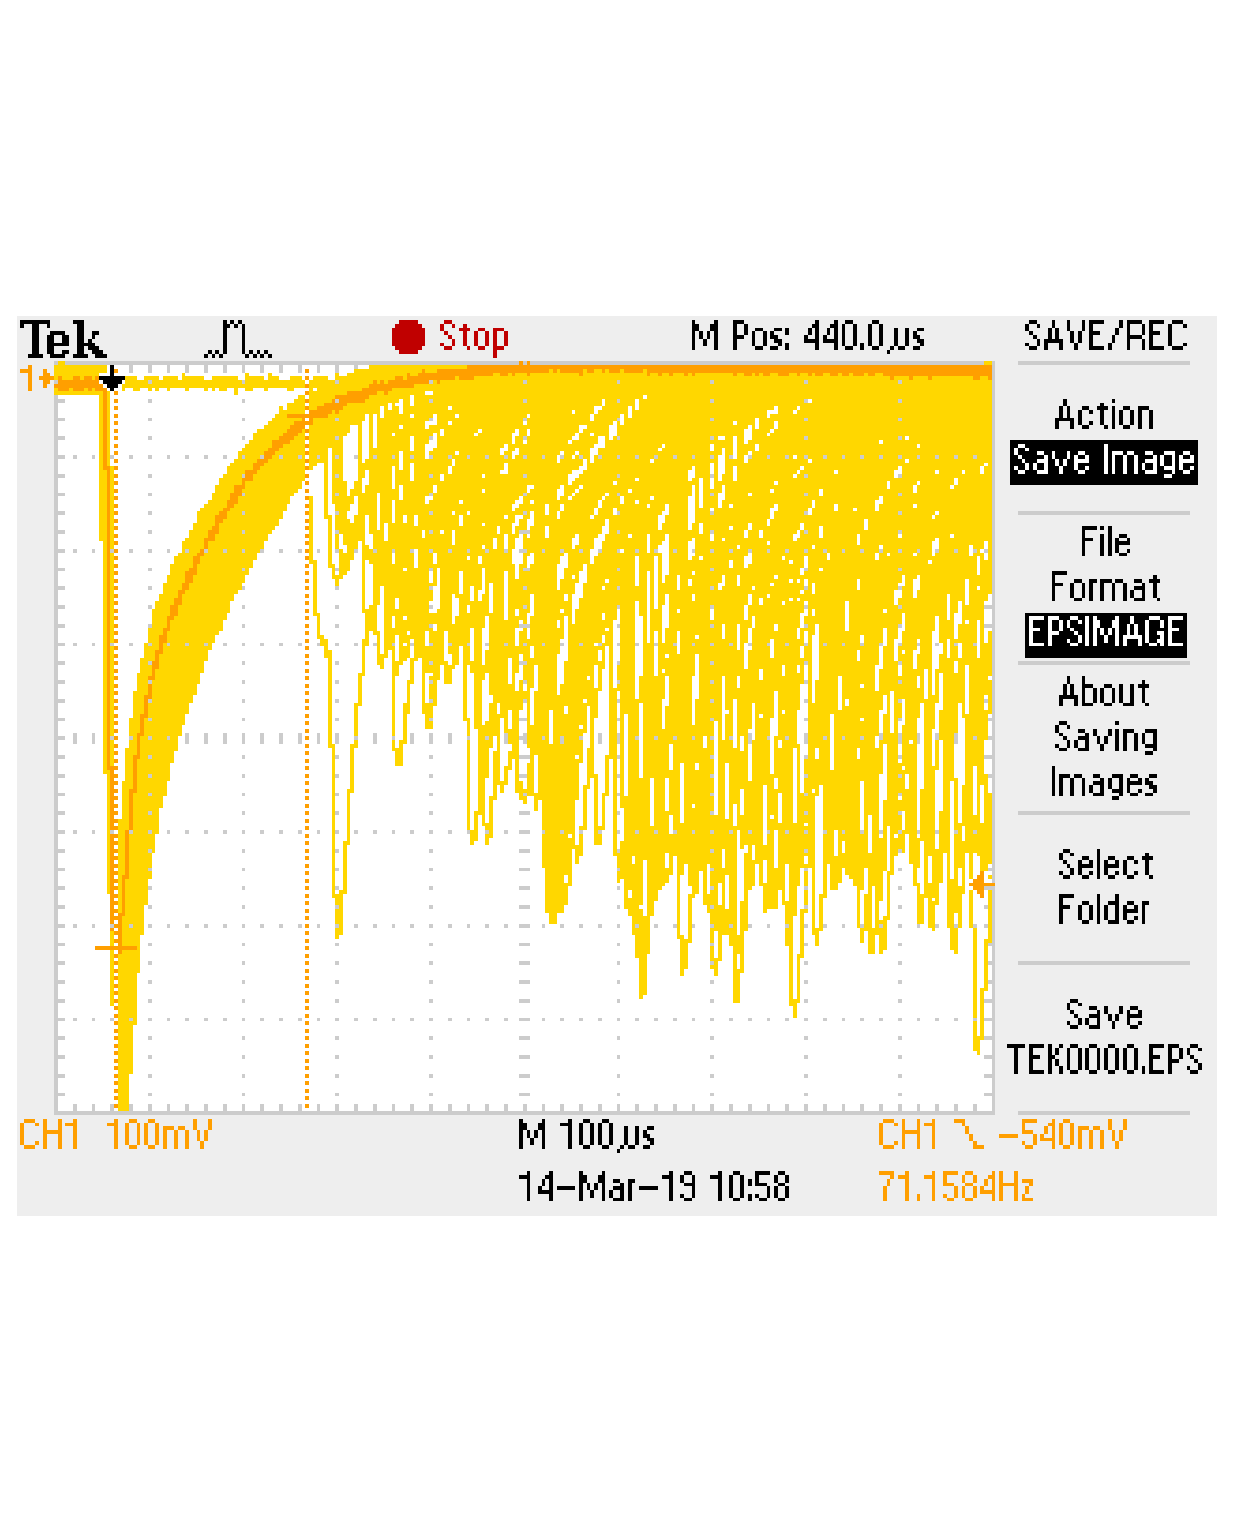
\includegraphics[width=\textwidth]{../Data/ALL0000/TEK0000.EPS}
%\caption{Stever diagram}
%\label{fig:Stever}
%\end{figure}

With a Stever diagram we can estimate the resolution time on the oscilloscope out of the dead time an the recovery time that we can read from the scope. 

The dead time is the distance between the main peak and the next incoming peak, during that time the GM-Counter can not detect anything.
We estimate the dead time with $\SI{224 \pm 4}{\micro s}$ (for that we read the dead time out of the steverdiagram 3 time with a min and max value and mean over all)
The recovery time is the distance bewteen main peak and the next main peak, we estimated it as $\SI{505\pm11}{\micro s}$ (same method as before).

\subsubsection{Characteristic curve of GM-Counter}
After the dead time correction we can now study the characteristic Geiger curve.
We plot the voltage (in 10 Volt steps) over the measured counts per 1s ($\frac{\mathrm{actual\,counts}}{10\,s}$).

With the calculated resolution time we can now correct the characteistic GM-curve for the detected counts with $N =\frac{n}{1-n\cdot\tau}$. 
For errors we used the uncertainties package for python, which calculates errors with gaussian propagation.

%\begin{figure}[H]
%\centering
%\includegraphics[width=\textwidth]{../Figures/%Geiger_characteristic_curves_with_deadcorect.pdf}
%\caption{GM-Characteristic}
%\label{fig:GeigerCorect}
%\end{figure}

\section{Measurement of statistical distributions}

\subsection{Procedure}

First we set the measurement, such that an average of at least 25 events were recorded per measurement, while the Sr-probe was in the detector. We found $10\,s$ to be a good interval. Then we measured the number of events per $10\,s$, 100 times.

Next we removed the probe from the chamber and set the measurement time, such that the average event count per measurement was at most 2. There we found $2\,s$ to be a good intervall. Then we measured the number of events per $2\,s$, 113 times.

Next we placed the probe in the chamber again and used the oscilloscope to take a shot of the pulses on a $50\,ms$ scale. We will use this data to measure the times between two consecutive events.

We repeated the last measurement with an alternative method: using the counter we recorded the counts per $0.1\,s$ 50 times.

\subsection{Analysis}

In \cref{fig:GaussHist} we see the recorded count rates for the Geiger counter with the Sr-probe in a histogramm, that vaguely resemble a gaussian distribution. We calculated the mean and standard deviation of our data and with those calculated our expected gauss distribution, according to
\begin{equation}
P(k) = \frac{1}{\sqrt{2\pi}\sigma} \exp(-\frac{(k-\mu)^2}{2\sigma^2}).
\end{equation}
This expected curve is shown in \cref{fig:GaussFit} together with the normalized histogramm of the count rates. In the same figure we also plotted a gauss curve we fitted with the least square method with $\mu$ and $\sigma$ as free parameters.

\begin{figure}[H]
\centering
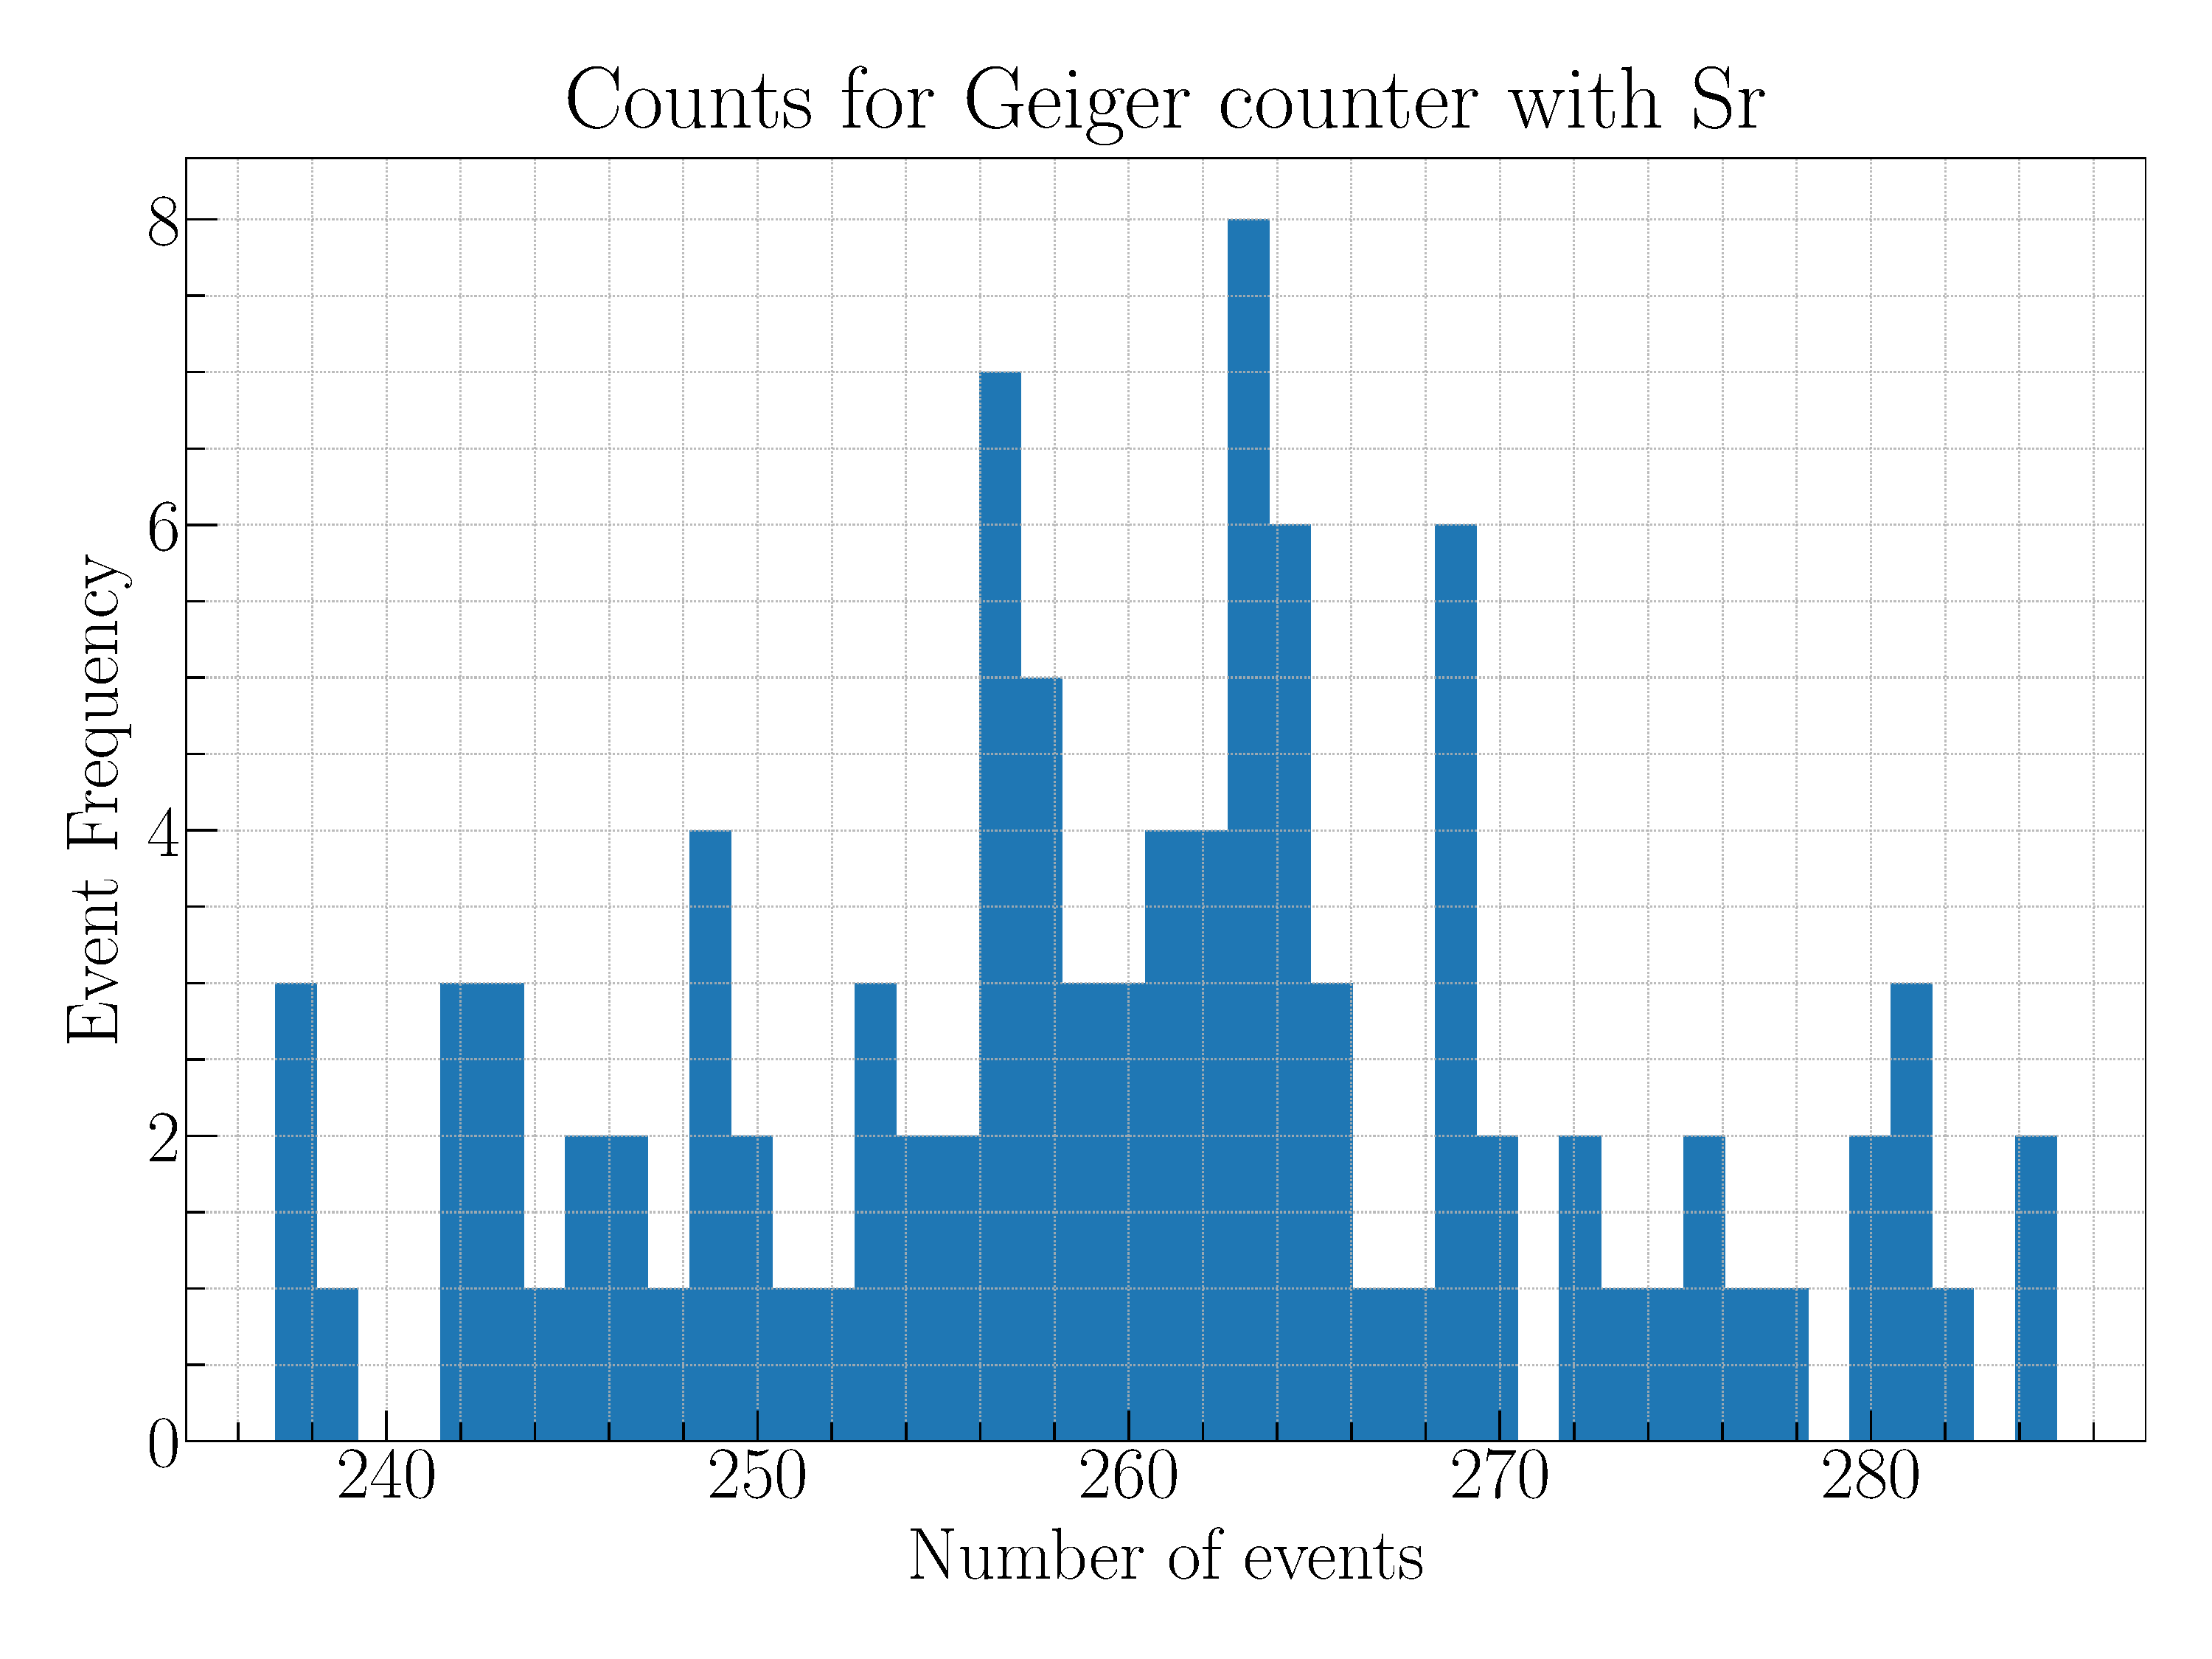
\includegraphics[width=\textwidth]{../Figures/Geiger_gauss_histogram.pdf}
\caption{gauss hist}
\label{fig:GaussHist}
\end{figure}

\begin{figure}[H]
\centering
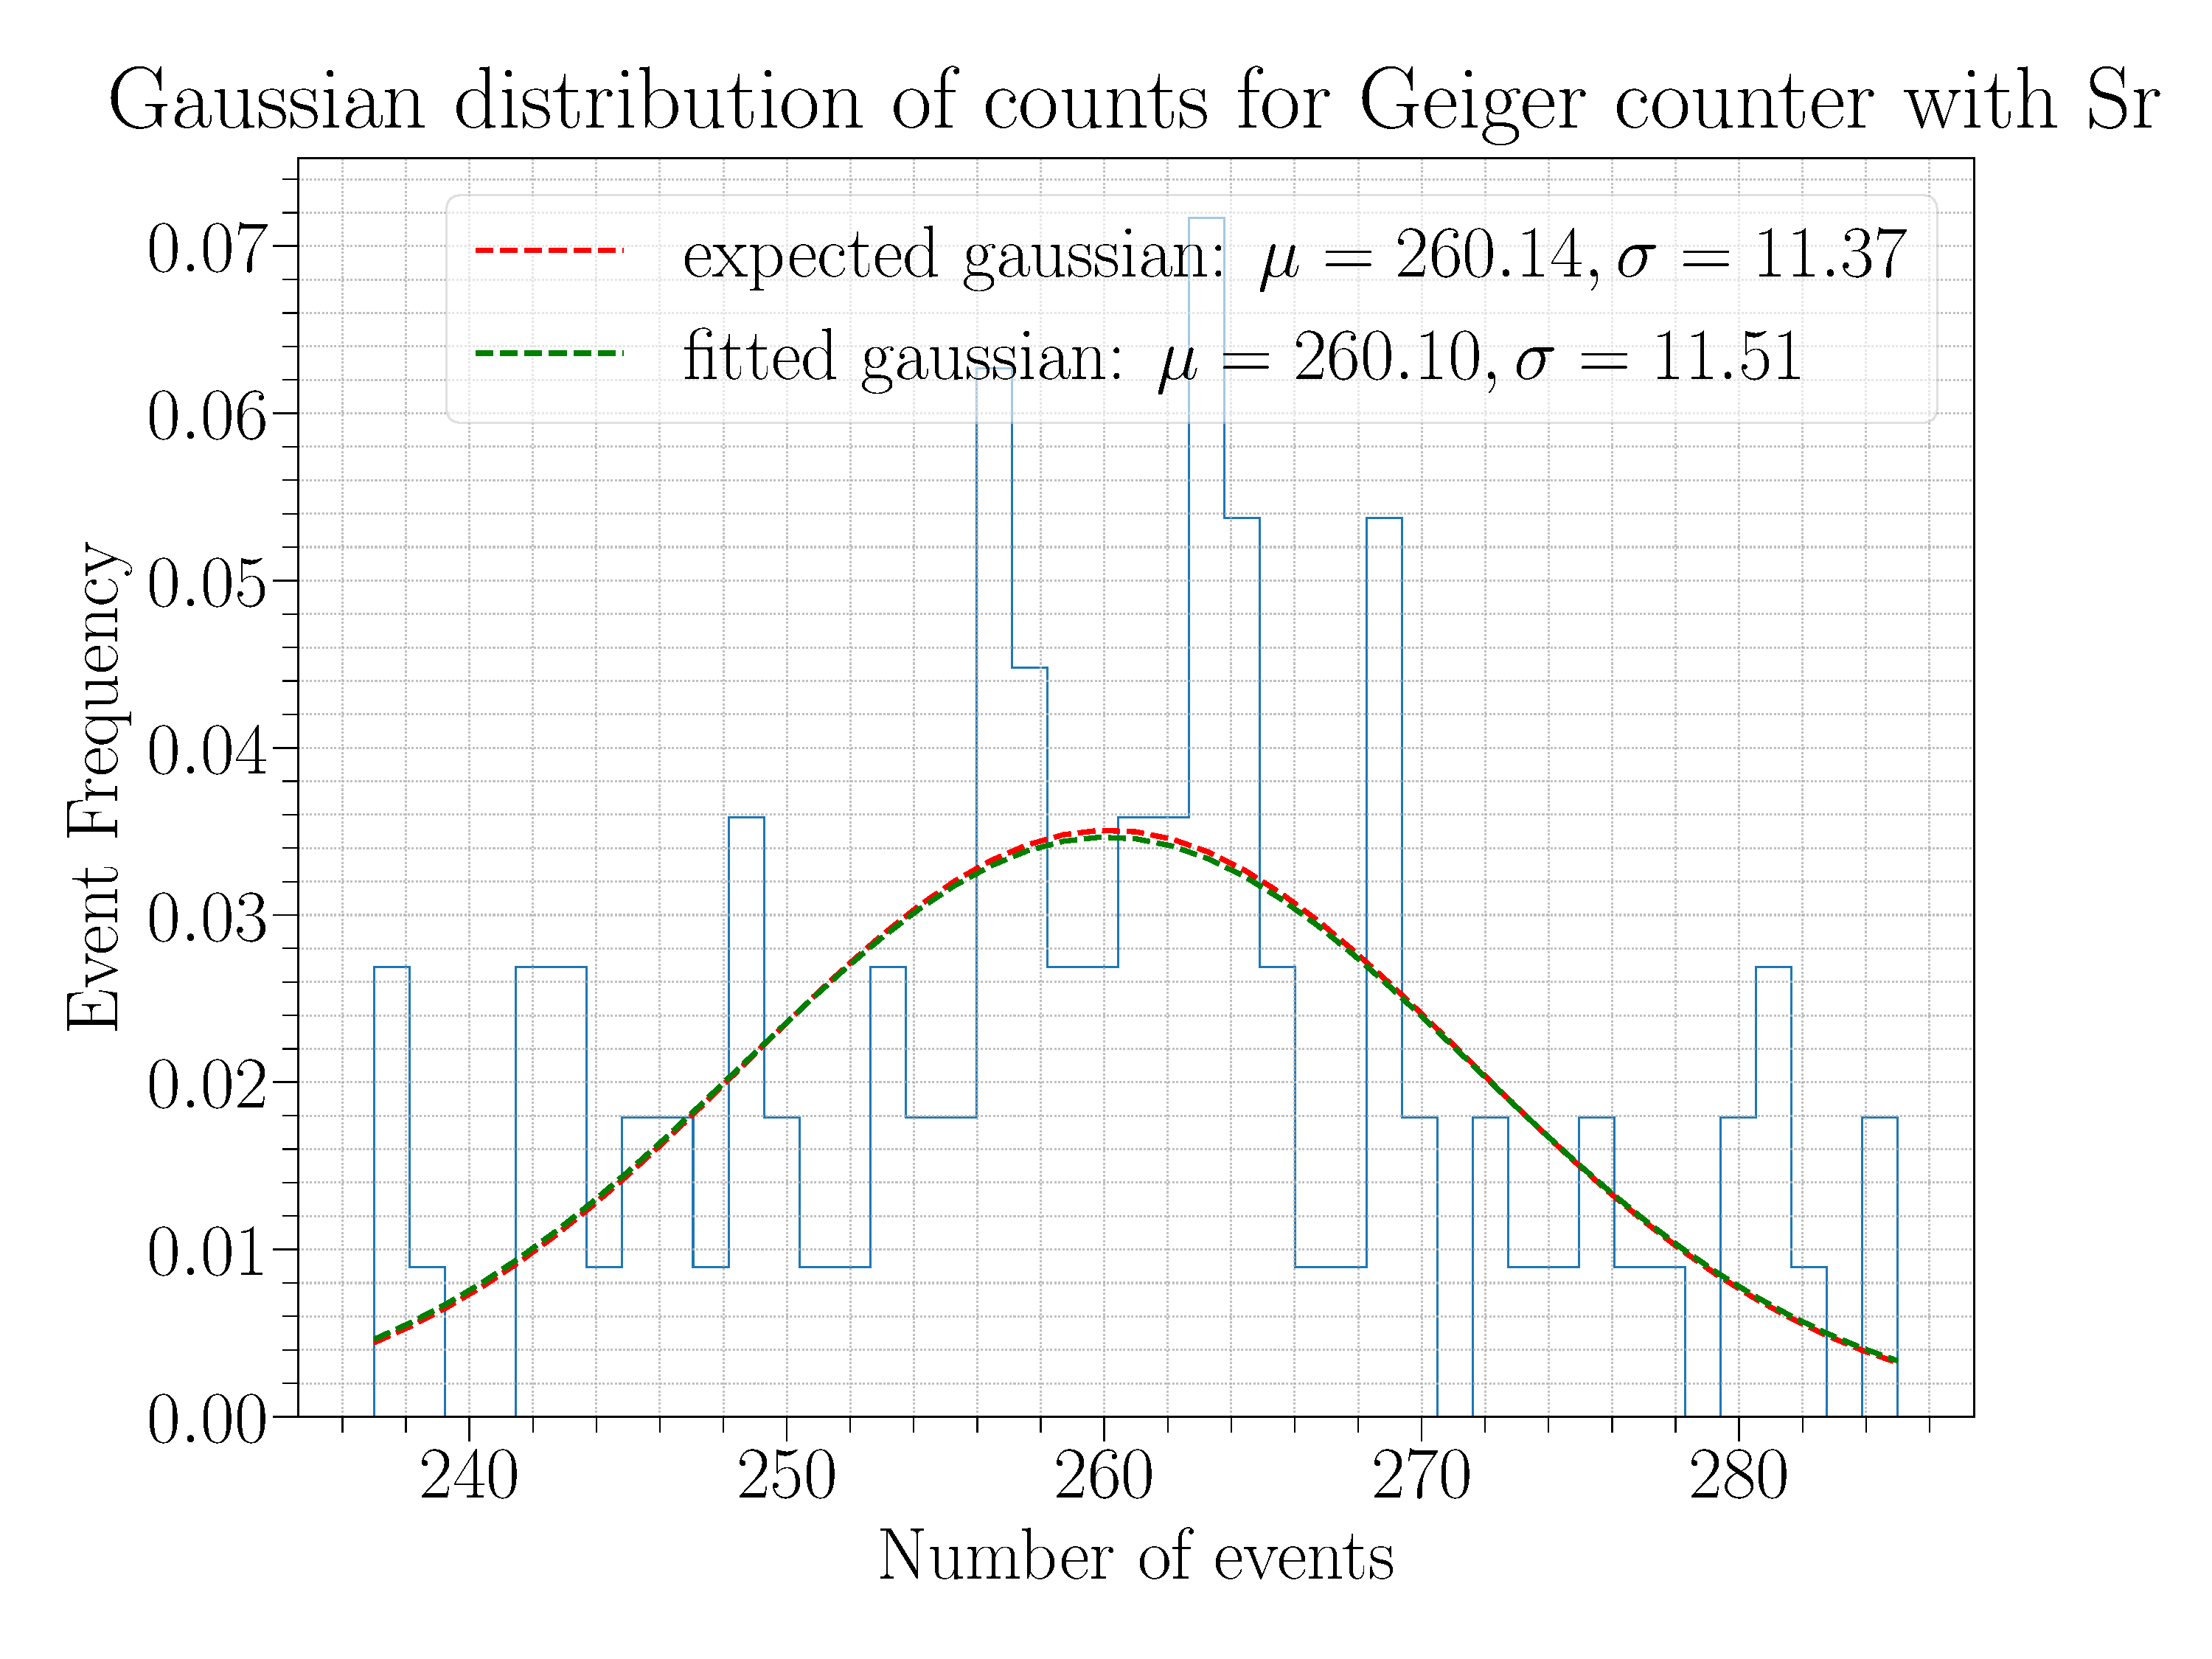
\includegraphics[width=\textwidth]{../Figures/Geiger_gauss_fit.pdf}
\caption{gauss fit}
\label{fig:GaussFit}
\end{figure}

We proceed analogously for the count rates of the empty Geiger counter. In \cref{fig:PoissonHist} we see the measured count rates and in \cref{fig:PoissonFit} we plotted the normalized histogramm, together with both the expected and the fitted poisson distribution
\begin{equation}
P(k) = \frac{\mu^k e^{-\mu}}{k!}.
\end{equation}
Of course here we only have one parameter, the mean value $\mu$, since the standard deviation is given by $\sigma = \sqrt{\mu}$.

\begin{figure}[H]
\centering
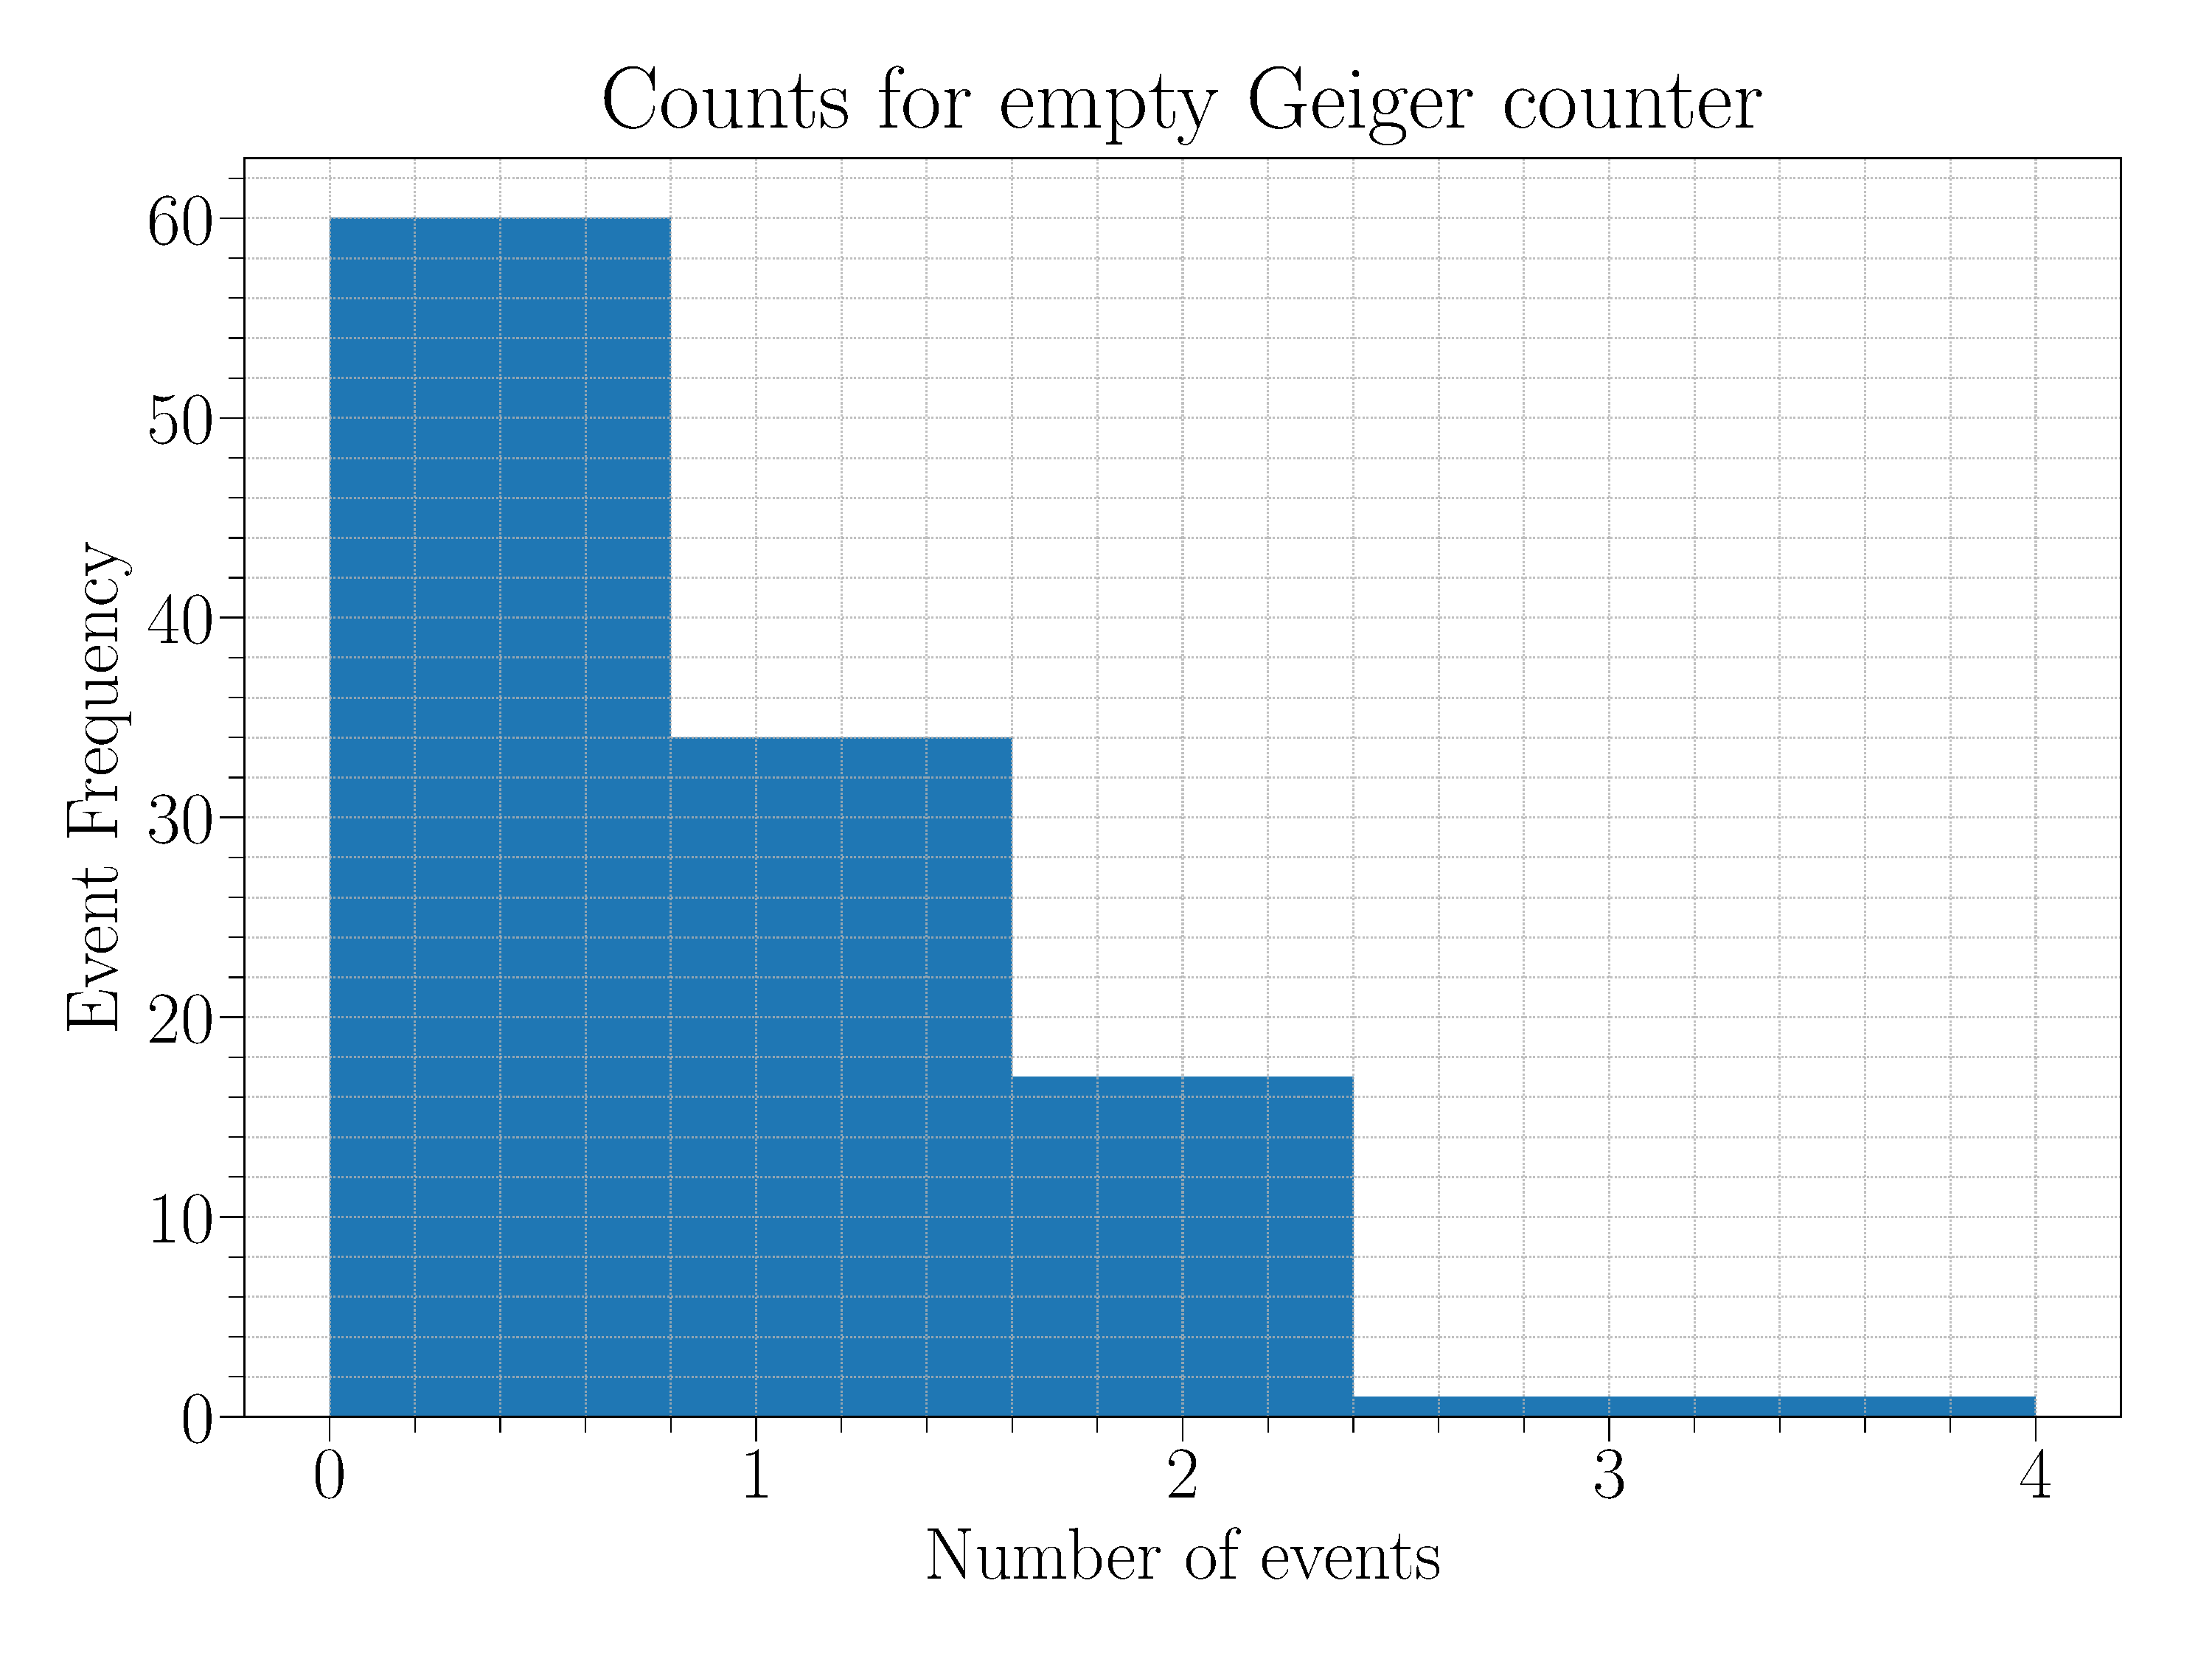
\includegraphics[width=\textwidth]{../Figures/Geiger_poisson_histogram.pdf}
\caption{poisson hist}
\label{fig:PoissonHist}
\end{figure}

\begin{figure}[H]
\centering
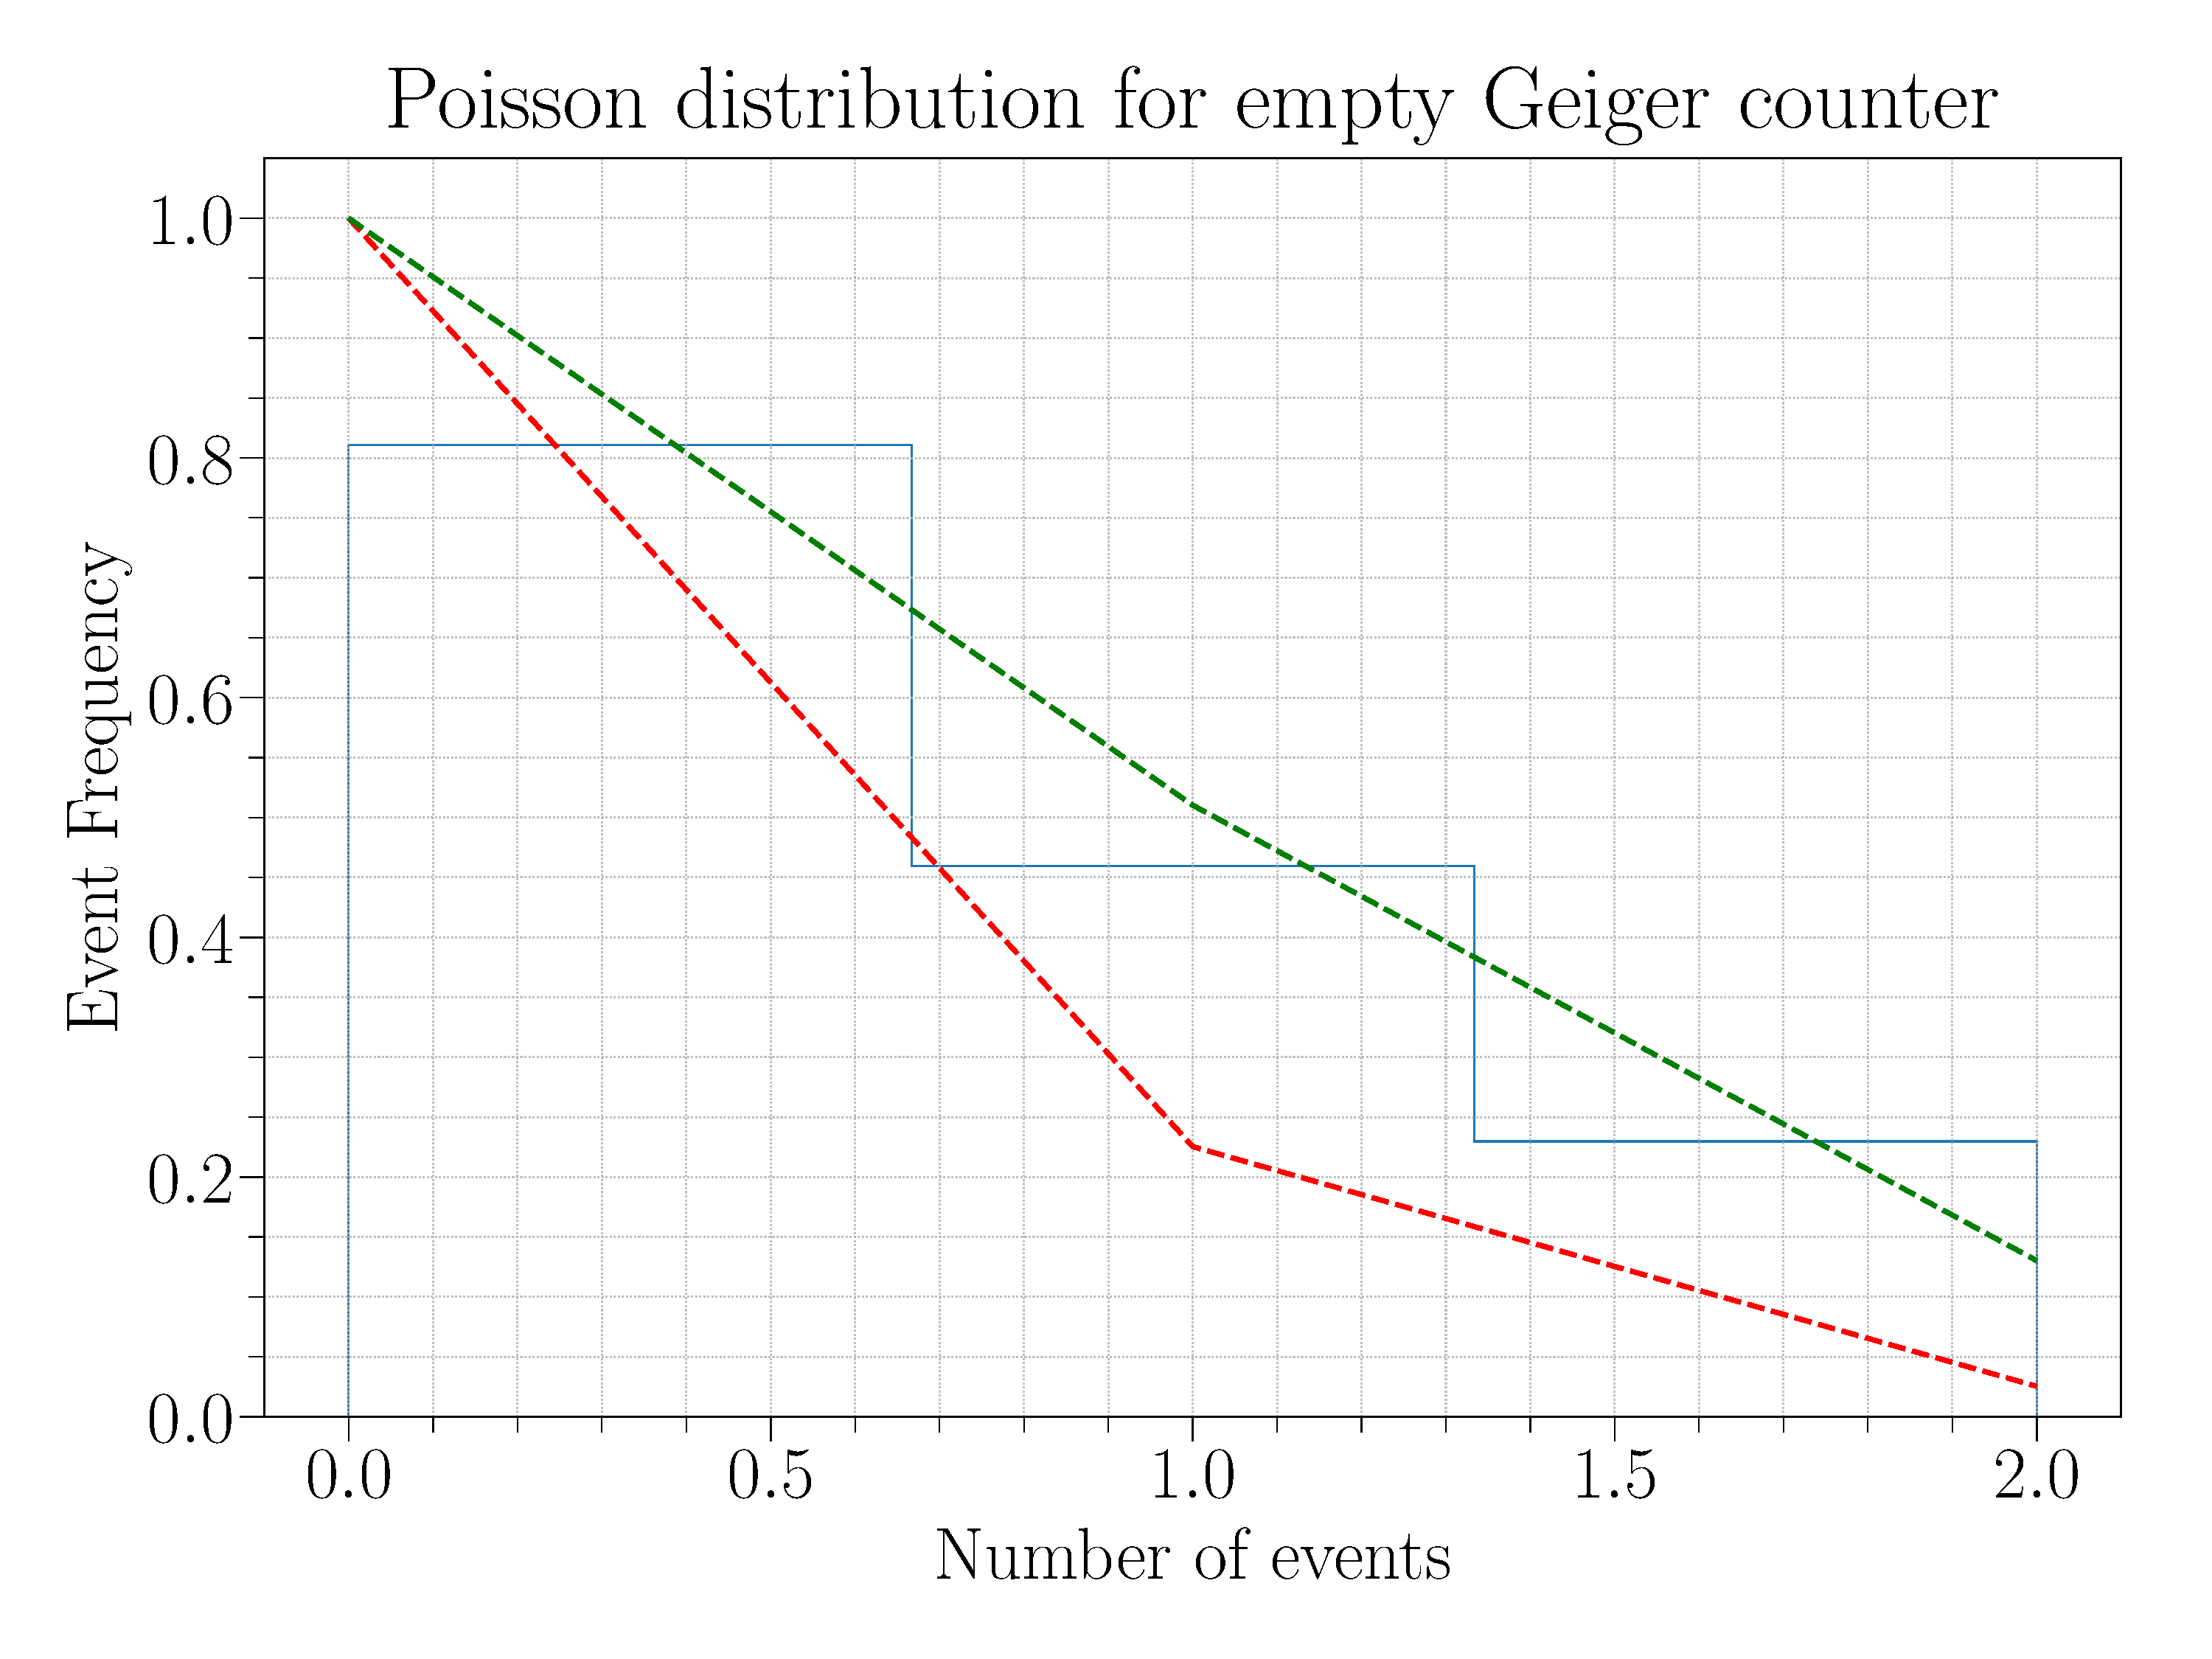
\includegraphics[width=\textwidth]{../Figures/Geiger_poisson_fit.pdf}
\caption{poisson fit}
\label{fig:PoissonFit}
\end{figure}

To test the goodness of our predictions, we did a $\chi^2$ test for all of the distributions.   

\begin{table}[H]
	\renewcommand{\arraystretch}{1.5}
	\centering
	\begin{tabular}{|c|c|c|c|}
		\hline
		Distribution & Parameter & Expected & Fitted \\
		\hline
		\multirow{2}{*}{Gaussian} & $\mu$ & \SI{260.14 \pm 1.14}{} & \SI{260.10 \pm 2.67}{} \\
		 & $\sigma$ & \SI{11.37}{} & \SI{11.51 \pm 1.86}{} \\
		\hline
		\multirow{2}{*}{Poisson} & $\mu$ & \SI{0.66 \pm 0.08}{} & \SI{1.14 \pm 0.20}{} \\
		 & $\sqrt{\mu}$ & \SI{0.81 \pm 0,05}{} & \SI{1,07 \pm 0,10}{} \\
		\hline
		\multirow{2}{*}{Exponential} & $\mu$ & \SI{}{} & \SI{}{} \\
		 & $\sigma$ & \SI{}{} & \SI{}{} \\
		\hline
	\end{tabular}
	\caption{Parameters for expected and fitted distributions.}
	\label{tab:DistPara}
\end{table}

\begin{table}[H]
	\renewcommand{\arraystretch}{1.5}
	\centering
	\begin{tabular}{|c|c|c|c|}
		\hline
		Distribution & Parameter & Expected & Fitted \\
		\hline
		\multirow{2}{*}{Gaussian} & $\chi^2$ & \SI{0.115}{} & \SI{0.119}{} \\
		 & $P$ value & \SI{0.944}{} & \SI{0.942}{} \\
		\hline
		\multirow{2}{*}{Poisson} & $\chi^2$ & \SI{1.02}{} & \SI{0.23}{} \\
		 & $P$ value & \SI{0.31}{} & \SI{0.63}{} \\
		\hline
		\multirow{2}{*}{Exponential} & $\chi^2$ & \SI{}{} & \SI{}{} \\
		 & $P$ value & \SI{}{} & \SI{}{} \\
		\hline
	\end{tabular}
	\caption{Goodness of expected and fitted distributions.}
	\label{tab:DistGood}
\end{table}

\section{Measurements with the proportional counter}

\subsection{Procedure}

\subsection{Analysis}

\section{Conclusion}



\end{document}
